\section{Analysis}
\label{sec:analysis}
\lhead{\thesection \space Analysis}

This chapter describes how the project's requirements and the customer's expectations are broken down in specific activities to reflect the behaviour of the software.
First all use cases are collected. Then the use cases are assigned to specific epics - a logical collection of use cases. Afterwards the resulting Software Requirement Specification for the first epic is presented. Finally a brief overview of the application architecture is given.

\subsubsection{Use Case Diagram}
\label{sssec:use_case_diagram}

The Use Case Diagram allows a quick overview of the main features the application has. It describes the activities that should be accessible to the different stakeholders.

\begin{figure}[H]
    \begin{center}
        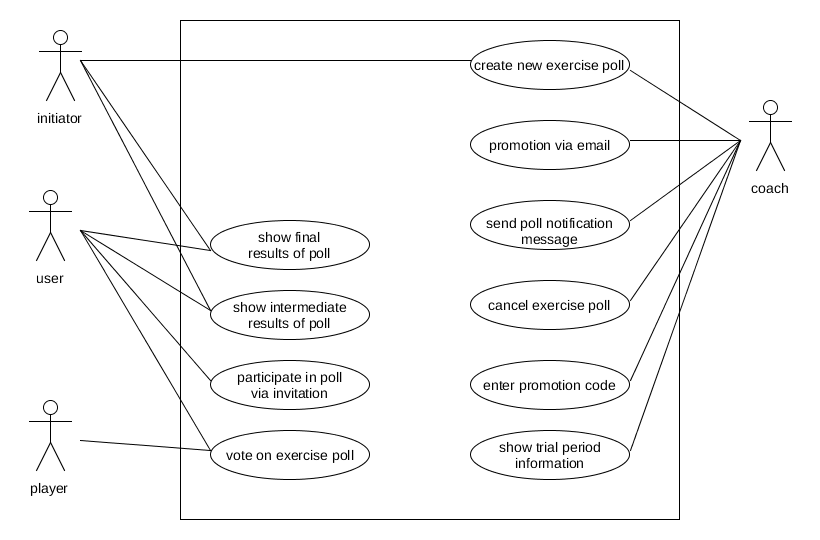
\includegraphics[width=\textwidth]{images/ucd.png}
        \caption{Use Case Diagram}
        \label{fig:ucd}
    \end{center}
\end{figure}

\subsection{Epics}
\label{ssec:epics}

To break down the development every use cases is assigned to a specific epic. An epic contains of use cases that have similar dependencies or depend on one another.

\subsubsection{Epic 1 - Vote4Fun}
\label{sssec:epic1}

The first epic includes the use cases needed to have a voting system for already registered users. They are allowed to vote on an exercise based on team membership and the coaches invitations of users by e-mail address.

The use cases relevant to the first epic are the following:

\begin{itemize}
    \item UC – 1.1 
    \newline
    Create new exercise poll.
    \item UC – 1.2 
    \newline
    Cancel exercise poll.
    \item UC – 1.3 
    \newline
    Vote on exercise poll.
    \item UC – 1.4 
    \newline
    Show final result of exercise poll.
    \item UC – 1.5 
    \newline
    Show intermediate result of exercise poll.
\end{itemize}

\subsubsection{Epic 2 - Promotion Code}
\label{sssec:epic2}
In addition to Epic 1, a coach user should be able to use a trial promotion code if he / she doesn't have the regular "\textit{VOTE4FUN}" feature to manage and start a \textit{Vote4Fun} poll for his / her team. 
\newline
This trial includes (a combination of):
\begin{itemize}
    \item A trial period in days
    \item A  maximum number of  voting polls to be created and managed
\end{itemize}
The period and number of polls for each trial code should be flexible. 
\newline
The trial code can be received via email with a \textit{promotion link, promotion code (string of characters)} or as a \textit{notification} on his /  her phone. 
\newline
\newline
The following requirements were given for this epic:
\begin{itemize}
    \item UR – 2.1 
    \newline
    A coach can open a view (position to be determined) to enter a trial code for managing Vote4Fun polls if and only if the user does not have the Vote4Fun permission.
    \item UR – 2.2
    \newline
    A coach can enter and submit a trial code.
    \item UR – 2.3 
    \newline
    A user receives a confirmation after entering the trial code.
    \item UR – 2.4 
    \newline
    A user receives a positive confirmation after entering a valid trial code.
    \item UR – 2.5 
    \newline
    A user receives a negative confirmation after entering an invalid trial code.
    \item UR – 2.6
    \newline
    A user can create and manage Vote4Fun polls after entering a valid trial code.
    \item UR – 2.7 
    \newline
    A user can see the remaining trial period / number of polls to be managed.
    \item UR – 2.8
    \newline
    A user with the app installed can click on an email promotion link to have the promotion code entered automatically.
    \item UR – 2.9 
    \newline
    A user with the app installed can click on a notification to have the promotion code entered automatically.
\end{itemize}

\subsubsection{Epic 3 - TODO Add Name}
\label{sssec:epic3}

TODO Patrick

\subsection{Application Architecture}
\label{ssec:application_architecture}

\begin{figure}[H]
    \begin{center}
        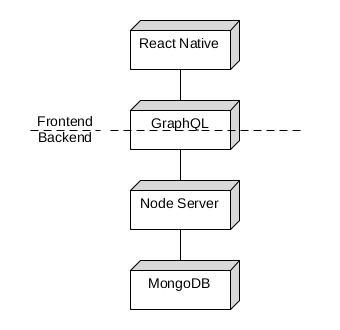
\includegraphics[width=\textwidth/2]{images/overview.png}
        \caption{Architecture Overview}
        \label{fig:architecture_overview}
    \end{center}
\end{figure}

The applications' frontend is based on \textit{React Native}, it uses \textit{GraphQL} to communicate with a node server saving its data in a \textit{MongoDB} database.

\subsection{Software Requirements Specification}
\label{ssec:software_requirements_specification}

TODO Marco